\documentclass[12pt]{article}
%\usepackage[utf8]{inputenc}
%\documentclass[UTF8]{ctexart}
%\usepackage[UTF8, heading = false, scheme = plain]{ctex}
\usepackage{geometry}
%geometry{a4paper,scale=0.9}
\geometry{a4paper,left=1cm,right=1cm,top=1cm,bottom=2cm}
\usepackage{amsfonts}
\usepackage{color}
\usepackage{url}
%\usepackage{biblatex}
\usepackage{amsmath}
\usepackage{amssymb}
\usepackage{latexsym}
\usepackage{cite}
%\addbibresource{ref.bib}
%\bibliography{ref.bib}
\usepackage{caption}
\usepackage{graphicx, subfig}
\usepackage{float}
%\usepackage[fontset=ubuntu]{ctex}
%\usepackage{fontspec}
\usepackage{xeCJK}
%\usepackage[colorlinks,
%anchorcolor=black,
%citecolor=black]{hyperref}
%\setmainfont{SimSun}
\usepackage[section]{placeins}
\usepackage{enumitem}
\usepackage{framed}
\usepackage[framemethod=TikZ]{mdframed}
\usepackage{indentfirst}
\usepackage{setspace}%使用间距宏包
\linespread{1.5}
%\title{预备知识}
%\author{leolinuxer }
%\date{June 2020}

\title{卷积\cite{Understand_Convolution}}
%\author{leolinuxer }
%\date{June 2020}

\begin{document}
\maketitle

\section{基础定义}
我们称$(f*g)(n)$为$f,g$的卷积。

其连续的定义为:
$$
(f*g)(n)=\int_{-\infty}^{\infty}f(\tau)g(n-\tau)d\tau
$$

其离散的定义为:
$$
(f*g)(n)=\sum _{\tau=-\infty }^{\infty}{f(\tau)g(n-\tau)}
$$

这两个式子有一个共同的特征:
$$
n = \tau + (n - \tau)
$$

如果我们令 $x = \tau, y = n - \tau$,那么 $x + y = n$,是一族斜率为$-1$的直线。如果遍历这些直线,就好比,把毛巾沿着角卷起来。或许,这就是“卷”积名字的来源吧。

\subsection{离散卷积的例子:丢骰子}
如果同时掷了两枚骰子,那么两枚骰子的点数加起来为$4$的概率是多少?

这里问题的关键是,两个骰子加起来要等于4,这正是卷积的应用场景。我们把骰子各个点数出现的概率表示出来:

其中,$f(1)$表示第一颗骰子掷出 $1$ 的概率;$g(1)$表示第二颗骰子掷出 $1$ 的概率。那么,两个骰子加起来等于4可以用下图表示:

\begin{figure}[H]
  \centering
  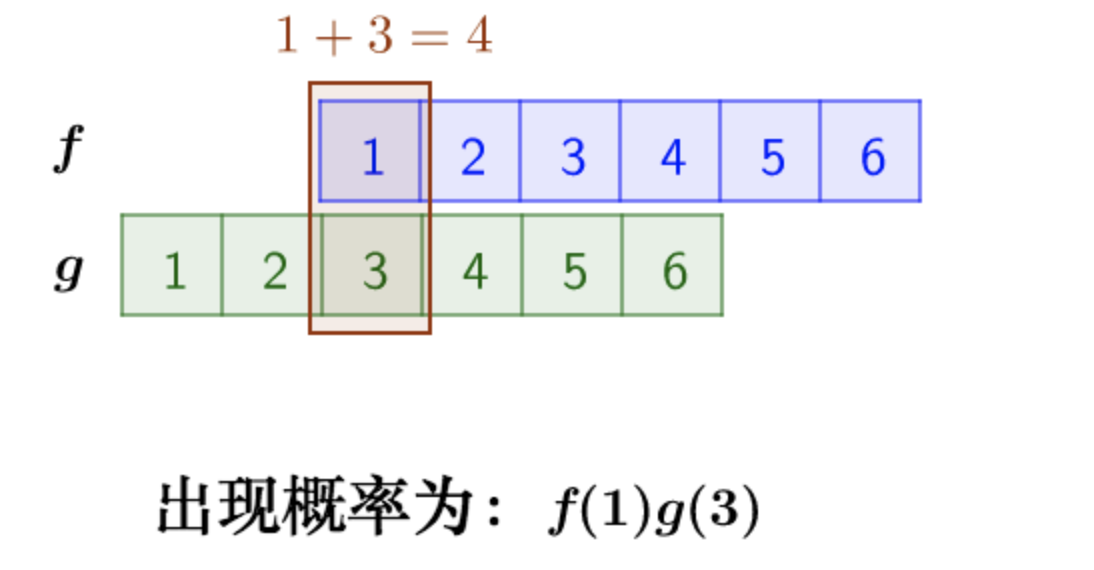
\includegraphics[width=.8\textwidth]{fig/convulution_two_dices.png} 
\end{figure}

即:两枚骰子点数加起来为4的概率为:
$f(1)g(3)+f(2)g(2)+f(3)g(1)$

符合卷积的定义,把它写成标准的形式就是:
$$
(f*g)(4)=\sum_{m=1}^{3}f(m)g(4-m)
$$

\subsection{连续卷积的例子:做馒头}
楼下早点铺子生意太好了,供不应求,就买了一台机器,不断的生产馒头。假设馒头的生产速度是$f(t)$,那么一天后生产出来的馒头总量为:
$\int_{0}^{24}f(t)dt$。

馒头生产出来之后,就会慢慢腐败,假设腐败函数为$g(t)$,比如,10个馒头,24小时会腐败:
$10*g(t)$

想想就知道,第一个小时生产出来的馒头,一天后会经历24小时的腐败,第二个小时生产出来的馒头,一天后会经历23小时的腐败。

如此,我们可以知道,一天后,馒头总共腐败了:
$\int_{0}^{24}f(t)g(24-t)dt$
这就是连续的卷积。

\subsection{在图像上的例子}
回忆一下在图像上,卷积的计算过程,也是符合卷积的公式的。

%\printbibliography
\bibliography{../ref}
\bibliographystyle{IEEEtran}
\end{document}

